% !TeX root = ../main.tex
% Add the above to each chapter to make compiling the PDF easier in some editors.

\chapter{Introduction}\label{chapter:introduction}

\section{Background}
Internet of Things (IoT) has become an emerging technology with the power of low priced computational units and cloud technology. There are thousands of different examples in the real world which are aiming at both the end-users and the industry. To achieve such applications or prototypes of these applications, hundreds or thousands of working hours should be spent by software developers to implement both embedded software and web services to serve for their needs. 

In most cases, the applications have similar capability needs in their required web-services with some little customization. The most basic capabilities, which any web services should have, can be listed as;
\begin{itemize}
  \item Receiving data,
  \item Serving data,
  \item Applying rules on gathered data when an event occurs,
  \item User authentication and authorization,
  \item Data isolation.
\end{itemize}
 Furthermore, they may need to support multiple protocols at the same time for accessing and modifying the same data since these web services should be accessible by different platforms. Although multiple protocols are used at the same time, the choice of protocols is always similar. 

 Message Queue Telemetry Transport (MQTT), Constrained Application Protocol (CoAP) and Hypertext Transfer Protocol (HTTP) in Representational State Transfer (REST) architectural style are the most used protocols in the area of IoT \cite{8246418,8070130}. Machine to machine (M2M) communications between wireless sensor network nodes and web application server are done through CoAP since they are resource-constrained devices in terms of the power source, the memory, and the network availability and CoAP is designed to be used in these kinds of constrained networks. If a node needs to send a message to multiple different nodes at the same time, MQTT is preferred since it is a lightweight publish-subscribe based messaging protocol and supports one-to-many communication \cite{mqtt}. Devices such as smartphones and personal computers which are not in a constrained network use HTTP in a RESTful way to monitor the gathered data and/or to start events.

 The common trait of all these protocols is being highly generic to support any needs of the developer on their communication through the internet. On the other hand, the required functionalities of web services that are used in the area of IoT diverge from each other with only a little difference. Interoperability of sensors, actuators, machine to machine (M2M) communication and context-aware services is the main concern of IoT \cite{6651222}. Therefore, a Platform as a Service (PaaS) can be defined to develop custom web services in IoT domain by using predefined and parameterized building blocks in order to give developers a fast and practical environment to work on.

\section{Proposed Solution}



While designing web services that will be used in an IoT project, some design concerns must be taken into account by the developer. The techniques and architecture to enable communication between all necessary nodes, the format for data that will be stored, how and when data will be served can be considered the main design concerns \cite{6651222}. After the design phase of the system has been finished, the design shall be easily translated to make web services up and running. 

M. G. Kibria et al. proposed that a semantic ontology which declares every device as objects on gateways can be used for energy efficiency \cite{7993747}. N. Lee and H. Lee also suggested an IoT service architecture provides services with an object gateway \cite{6884496}. Although device objectification is a good method to store data of the real world devices for IoT services; the management of read-write access to the objects, the evaluation of the gathered data and the methods for the service of these data are the topics need to be covered to build a generic and practical platform that serves any need of IoT. 


To achieve a PaaS that enables a fast, practical, accessible and generic environment that can support any IoT developer, different subsystems that handle different objectives in the system must be defined. By having different subsystems,  isolation of information and a system that scales only its required subsystems can be succeeded. On the other hand, the challenge of interoperability between these subsystem derives. In figure \ref{fig:architecture}, the architectural design of the system is shown.

\begin{figure}[htpb]
  \centering
  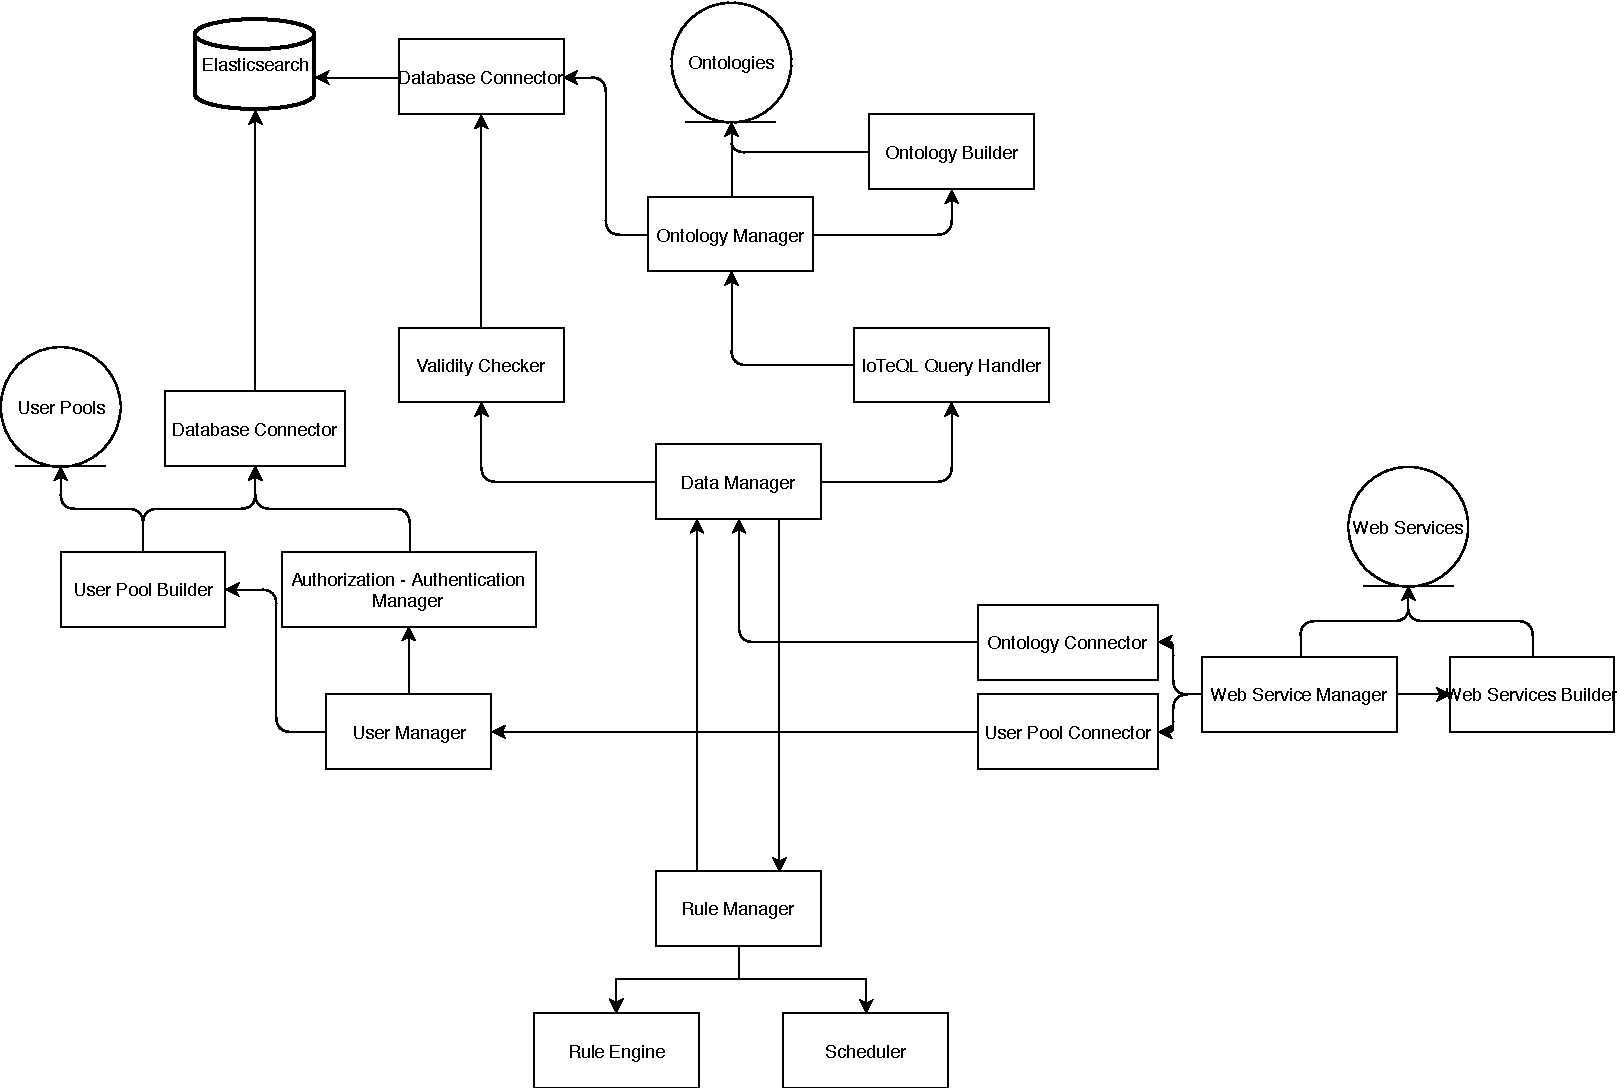
\includegraphics[width=\textwidth,height=\textheight,keepaspectratio]{figures/architectural_diagram.pdf}
  \caption[Platform Architecture]{The architectural diagram of the platform}\label{fig:architecture}
\end{figure}

Each of the subsystems; the user manager, the data manager, the rule manager and the web services manager are dockerized and hosted in different computing units in the cloud infrastructre. Since they are isolated and loosely coupled with each other, they can autoscale individually behind a load balancer and increase of the computational unit where there is needed can be achieved. Thus, the data manager will scale horizontally when number of queries is increased and the rule manager will scale horizontally when huge amount of scheduled rules is need to be handled at the same time. All of the subsystems can be accessed by their own application program interface (API) and the connector components of them act like adapter to interact with each other. Therefore, any change in any subsystem will not lead change in overall architecture. How to handle the interoperability challenges will be covered in the following chapters in details.


\subsection{Data Manager}

All the data that is defined by the platform user and the web service users is handled by the data manager and its components. Data manager uses Elasticsearch to store this data since its scalability, speed, resiliency, flexibility, powerful support to time-series and unstructured data and queries \cite{elastic, elastic_time}.

Any data that will be used by the web services that are defined by the platform user are stored as ontologies in the platform. These ontologies store different types of components as follows:

\begin{itemize}
  \item Types
  \item Figures
  \item Objects
  \item Groups
  \item Rules
\end{itemize}

The data model of an ontology is defined by types and figures and the actual data is defined by objects and groups. Each type has a name and abstract meta-data about data fields such as requirement, name, and type which will be used while defining objects. A type can be inherited by another types and figures or can be used to define objects. Figures are just like types, but, with predefined data fields. Objects that are defined by using a figure cannot alter these predefined data fields other than the value given in figures. Each figure cannot be inherited by a type and must inherit from a type. Each object is defined by using a type or a figure, represents the virtual state of the real-world object and can have concrete data, data series or rules that are defined in type or figure the object inherits and return on-time calculated value in its fields. To state a property or the state of the object, data fields can be used. However, data series are preferred to store a collection of the same type of data of the same object such as timestamped data of hourly energy consumption of a device. Groups are used to cluster objects and apply rules on objects as a cluster. Rules are chains of function blocks to apply on objects or groups when an event occurs. They are stored in ontologies with other components by the data manager. However, processing and handling of them are done by the rule manager. In the subsection \ref{ss:rule_manager}, the detailed information about rule structure will be given.

Any ontology owned by a platform user can be shared with other platform users to work collaboratively. Nevertheless, the platform users that have no access to an ontology are not allowed to view or modify the ontology. As a result, protection of business logic and private data will be preserved. Isolation management of ontologies is handled by the data manager. 

The created ontologies can only be organized and extended by the platform user. Any rules or object in an ontology will not function until the ontology is matched with a web service using the web service manager. Thus, an ontology that is not matched with any web service is considered offline and act like static data in the platform.

To enable reusability of an ontology, they can be edited, cloned or taken offline. Moreover, they can be matched with multiple web services and any changes made using a web service will be available on other matched web services. Therefore, the data will be available for the user-defined system from any kind of network.

The whole ontology can be defined in the practical and easy-to-learn user interface (UI) of the web application. However, the power users who want to transfer existing data models as ontologies to the platform with help of a script, to modify the ontology components that cannot be modified by the rules such as creating or removing rules with their own system or need to create a similar ontology with the small but core changes which would lead the loss of data when is done in UI can use Internet of Things Easy Query Language (IoTeQL) that is designed for querying the ontology model and enables all functionality of the ontology model for the needs of the user in a practical way. All queries on the ontologies are evaluated by the query engine component of the data manager. The detailed information and syntax of IoTeQL can be found in upcoming chapters. %TODO Chapter 


\subsection{Rule Manager}
\label{ss:rule_manager}

To build business logic on the ontologies, the rules, which are if-then form decision-making tools, must be defined in the platform. The rules function like a chain of blocks, which each takes a small part while interpreting the logic. These blocks send objects in JavaScript Object Notation (JSON) format to each other using their input and output ports. There are different types of blocks that each has a different function in the rule handling. In the following part, the blocks and their respective descriptions can be found.

\begin{description}
  \item [Nodes] are used to retrieve data from other components of the ontology. They can represent a type, a figure, an object or values in the data fields of the object. They are also directly accessible by the endpoints of a web service.
  \item [Queries] are used to create a new object or to modify the existing ones. They can match with the objects as a whole or as part of them and outputs state of the whole object. 
  \item [Sinks] are also used to connect the rules to the web services. They are the exit points for the data to be sent through the web services.f
  \item [Sources] are used to connect the rules to the web services. They are the entry points for the data received from the web services.
  \item [Events] are used to run the rules when a condition satisfied. This condition can be satisfied by time or other rule blocks. If the condition is time-based, they can run their respective rules with predefined value output at scheduled times. If it is expected to be triggered by other function blocks, they must have a condition to apply on input and outputs input to its target when the condition is satisfied.
  \item [Mappers] have a lambda function to apply every single element of the input and output elements which the function returns.
  \item [Reducers] have a lambda function which does rolling computation to apply to sequential pairs of data series.
  \item [Filters] have a lambda function which returns a boolean type value. They apply the lambda function to elements in the input and output elements which the function returns true.
  \item [Zippers] are used to merge more than one inputs into a single output.
  \item [Branchs] have more than one output ports and each output port have their respective condition. They forward their input to the output port or ports that conditions are satisfied.
  \item [Functions] are used to do a customized modification, when the capabilities of other blocks are not enough, on the input in a sequential programming way and output result.
\end{description}

 A web service triggers respective source in a rule on each request and returns the value received from sinks if it has one. The only way to run a rule is triggering its starting sink or event. Every rule block can have only one output port and can have more than one input ports except sinks and sources and are reusable with their target blocks by referencing them while creating a rule. With the power of reusable blocks, the platform user will not need to implement the rule parts that are implemented in other rules.

\subsection{User Manager}

The web services that are defined by the platform user may have public or private endpoints. To be able to reach the private endpoints, the web service user must have correct access rights. User pools can be defined by the platform user to manage access rights to private endpoints of the web services. The authorization rights, the user groups with assigned authorization rights and users which belong to one or more user groups and have personal information. 

The reason to keep the web services and the user pools separate is to escalate the reusability of the same user pool. The platform user may want to introduce new web services to his/her own system. In such a case, it would be undesirable for the web service users to create new accounts to use a new web service. Therefore, using the same user pool in both web services would be ideal. 

The new user pools can be created and managed through the web application. The endpoints of the REST API of the user pool are also provided to the platform user. With help of these endpoints, they can integrate user creation and modification functions for their users in different user groups to their own system. 

The user pools can also different user confirmation level. These confirmation levels define when the web services user needs to confirm they agree to use of their data in the web services. The objects that are owned by the web service user cannot be accessed with the web services on the ontology unless they give the permission. The confirmation to use the user information in any web services that are created by the owner at the creation of the web services user of the user or the confirmation need before the start of using of any individual web services can be set by the platform user for each user pool. The ease of handling of user data can be achieved by using needed user confirmation level for the platform users who are building web services in different countries with different user data protection regulations.


\subsection{Web Service Manager}

The web service manager is the backbone of all the system which integrates and manages the interoperability of all subsystems.  

While creating a web service using web service manager, the platform user must select which an ontology and a user pool will be used for the web service. The decision for the protocol that the web service will be built on must be made before the start of the creation of the endpoints. 

The access permission of the user groups for the endpoints, the protocol specific configuration of the endpoints and the matching between the endpoints and the sources or the nodes in the ontology must also be defined by the platform user during the creation of each endpoint. In protocols with the publish-subscribe mechanism, sinks must be matched with topics. Thus, the web service can listen for requests in topics which are matched with source and send responses in topics which are matched with responses.

When a web service user makes a request to the web service built-on protocols that have no publish-subscribe mechanism, the manager checks whether the web service user is in required groups and has been confirmed to be used in the web services as the user confirmation level of the user pool required. The web services with publish-subscribe mechanism make these checks while the web service user is subscribing to a topic. Unless any other specification is made by the platform user, web service manager will merge the user information, the query and the parameters sent by the web service user into one JSON object pass it to data manager to be handled by rule engine and returns the merged result in the all reached sinks. 
